\documentclass[a4paper,11pt]{article}
\usepackage[a4paper,bindingoffset=0in,left=0.9in,right=0.9in,top=1in,bottom=1in,footskip=.25in]{geometry}
\usepackage{generic}
\usepackage{booktabs,array}
\usepackage{graphicx}
\usepackage{amsmath,amssymb,amsfonts,amsthm}
\usepackage{setspace}
\usepackage{cite}
\usepackage{enumitem}
\usepackage[justification=centering]{caption}
\usepackage[colorlinks=true,linkcolor=blue,citecolor=blue,urlcolor=blue]{hyperref}
\usepackage[capitalize]{cleveref}
\setlist{noitemsep,topsep=0pt}
\setlength{\parindent}{0pt}
\setlength{\parskip}{6pt}
\setlength{\emergencystretch}{2em}
\renewcommand{\topfraction}{.9}
\renewcommand{\bottomfraction}{.9}
\renewcommand{\textfraction}{.05}
\renewcommand{\floatpagefraction}{.8}
\graphicspath{{figures/}}
\newtheorem{proposition}{Proposition}[section]
\title{Classical and Bayesian estimation of multicomponent stress-strength reliability for the Weibull distribution}
\author{Vaidik Maheshwari (250150045) \& Anant Gupta (250150004)\\[4pt]\small Mehta Family School of Data Science and AI, IIT Guwahati, India}
\date{}
\begin{document}
\begin{singlespace}
\maketitle
\end{singlespace}
\begin{abstract}
We study a system that works when at least three of five component strengths exceed a common random stress. Strength and stress follow Weibull distributions with the same shape and different rates. Strength observations are collected in blocks under progressive hybrid censoring, and stress observations are upper k-record values. We derive the reliability function and estimate it by unrestricted and order-restricted maximum likelihood. We also obtain Bayesian estimates under a dependent gamma-Dirichlet prior. A Monte Carlo study with 48 scenarios and 300 replications per scenario compares absolute bias and mean squared error. Asymptotic, equal-tail and numerical highest posterior density intervals are compared through coverage and average width. An incorrect order restriction increases bias and can prevent intervals from covering the true reliability. Published jute-fibre and carbon-fibre measurements illustrate the methods. The jute example has a Weibull-fit limitation; the additional carbon example is compatible with the fitted model.

\textbf{Keywords:} Weibull distribution; stress-strength reliability; progressive hybrid censoring; upper k-records; maximum likelihood; gamma-Dirichlet prior.
\end{abstract}

\section{Introduction}\label{sec:introduction}
Reliability is the probability that a system performs its intended task. In a stress-strength model, a component works when its strength is greater than the stress applied to it. A system with several components can continue to work even if some components fail. Here we consider an $s$-out-of-$K$ system: at least $s$ of the $K$ strengths must exceed the same stress.

Complete observations are not always available in a life test. Some specimens may be withdrawn before failure and the experiment may end at a time limit. Progressive hybrid censoring describes these two features. A block represents a separate test facility. For the stress sample, we retain upper k-records instead of every observation. These records are dependent, so their likelihood differs from the likelihood of independent Weibull observations.

Sultana et al.\ \cite{Sultana2026} study block Type-I hybrid censored Weibull populations, including order-restricted inference and a dependent prior. Newer \cite{Newer2025} combines block adaptive progressive hybrid censoring with upper k-record sampling for another distribution. Newer and Alanazi \cite{NewerAlanazi2026} discuss multicomponent reliability, Bayesian estimation and bootstrap inference under a different sampling design. We use these papers to develop the assigned Weibull model. We do not use their other distributions or ranked-set likelihoods in place of the model below.

The order assumption in this project is that the strength population is stochastically larger than the stress population. It can improve estimation when it is correct, but it can also produce misleading results when it is false. We therefore include correctly ordered, boundary and incorrectly ordered cases in the simulation. Sections~\ref{sec:mle} and~\ref{sec:bayes} present the classical and Bayesian estimates. Section~\ref{sec:numerical} contains the simulation and the data examples. Section~\ref{sec:conclusion} gives the conclusions.

\subsection{Weibull model and system reliability}\label{sec:model}
Let $X_1,\ldots,X_K$ be independent strengths, and let $Y$ be a stress independent of them. All strengths have rate $a$ and stress has rate $b$, with common shape $\alpha>0$. For a positive Weibull variable with rate $\lambda>0$,
\begin{align}
f(z;\alpha,\lambda)&=\alpha\lambda z^{\alpha-1}e^{-\lambda z^\alpha},\qquad z>0,\label{eq:density}\\
F(z)&=1-e^{-\lambda z^\alpha},\qquad S(z)=e^{-\lambda z^\alpha},\label{eq:survival}\\
h(z)&=\alpha\lambda z^{\alpha-1},\qquad
F^{-1}(u)=\left[\frac{-\log(1-u)}{\lambda}\right]^{1/\alpha}.\label{eq:quantile}
\end{align}
The usual scale is $\lambda^{-1/\alpha}$. We call $\lambda$ a rate to make the order assumption clear: $a\le b$ means that strength has greater survival than stress at every positive threshold. The shapes below and above one give decreasing and increasing hazards, respectively.

Conditional on $Y=y$, the number of surviving components is binomial with probability $e^{-ay^\alpha}$. Thus
\begin{equation}
R_{s,K}=\int_0^\infty\sum_{j=s}^K\binom Kj e^{-jay^\alpha}(1-e^{-ay^\alpha})^{K-j}f_Y(y)\,dy.\label{eq:reliability-integral}
\end{equation}
Put $\rho=b/a$ and $u=e^{-ay^\alpha}$. Since $f_Y(y)dy=-\rho u^{\rho-1}du$, integration gives
\begin{equation}
R_{s,K}=\rho\sum_{j=s}^K\binom Kj B(\rho+j,K-j+1).\label{eq:beta-reliability}
\end{equation}
An equivalent expression is easier to evaluate. The transformed strengths $X_i^\alpha$ are exponential with rate $a$. The $(K-s+1)$-th smallest transformed strength is a sum of independent exponentials with rates $Ka,(K-1)a,\ldots,sa$. Taking its Laplace transform at $b$ gives
\begin{equation}
\boxed{R_{s,K}=1-\prod_{j=s}^K\frac{j}{j+\rho}.}\label{eq:reliability}
\end{equation}
For $K=s=1$ this reduces to $b/(a+b)$. Reliability tends to zero as $\rho\to0$ and to one as $\rho\to\infty$. It does not depend directly on the common shape, although the fitted rates do. We use $s=3$ and $K=5$ throughout the numerical study. In this case $R_{3,5}=1/2$ at $a=b$, and the order restriction implies $R_{3,5}\ge1/2$.

The common stress in \eqref{eq:reliability-integral} matters. Component survival indicators are independent conditional on $Y$, but dependent after averaging over $Y$. Substituting $P(X>Y)$ directly into an ordinary binomial probability would describe a different experiment. The notebook checks \eqref{eq:reliability} by numerical integration and direct simulation.
\begin{figure}[htbp]
\centering
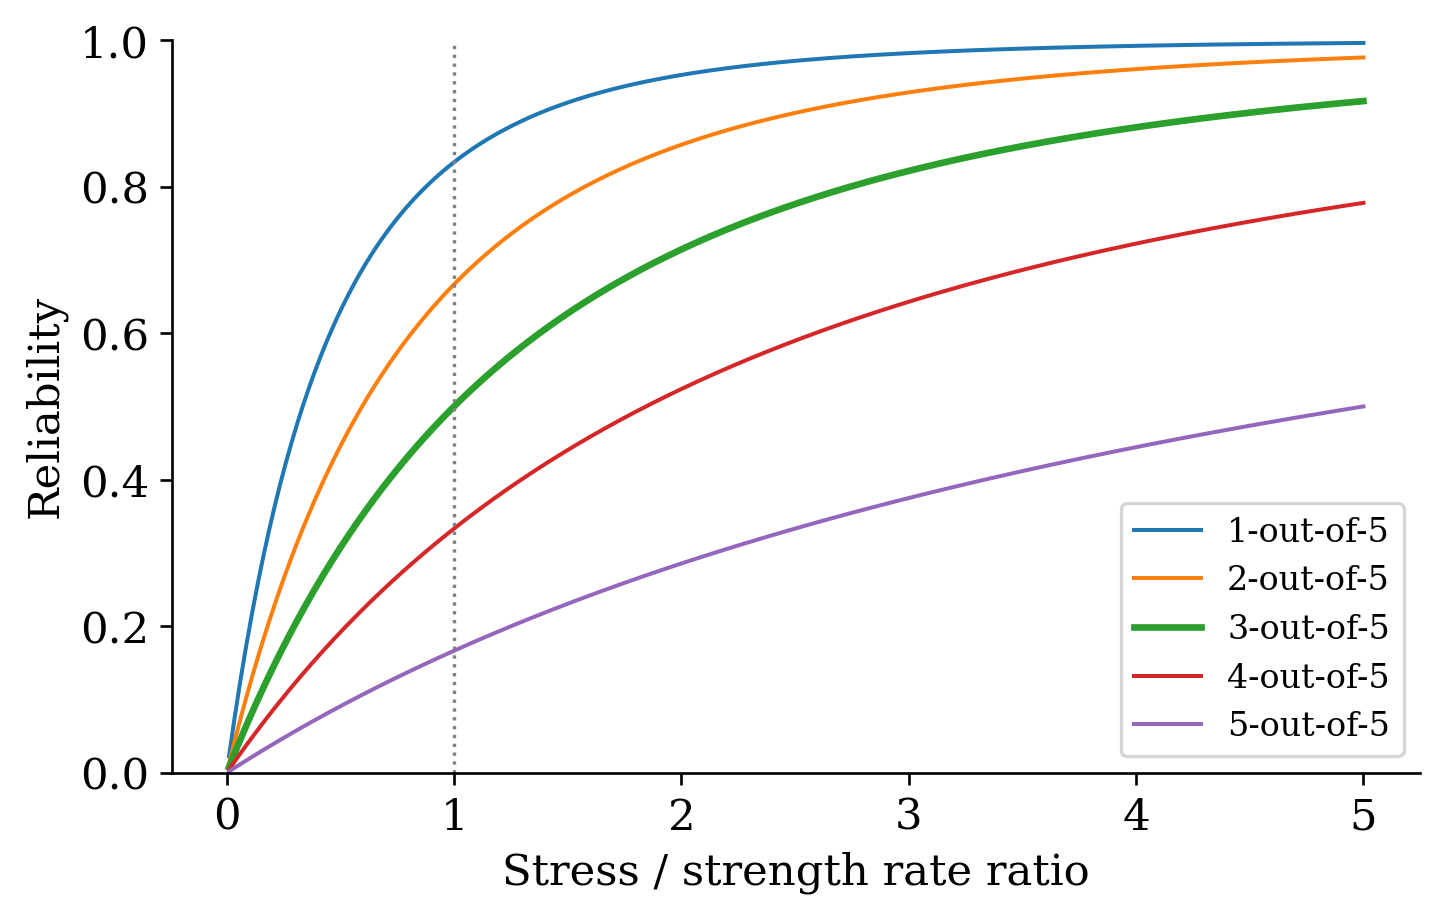
\includegraphics[width=.78\linewidth]{reliability.png}
\caption{System reliability as the stress-to-strength rate ratio changes. Each curve represents one value of $s$ with $K=5$.}\label{fig:reliability}
\end{figure}

\subsection{Observation schemes and likelihood}\label{sec:sampling}
For strength block $i$, start with $n_i$ specimens. Choose a target number of failures $m_i$, a time $T_i$, and planned withdrawals $R_{ij}$ satisfying $\sum_jR_{ij}=n_i-m_i$. Withdraw survivors uniformly, independently of their unobserved failure times.

The principal Type-I scheme stops at $\tau_i=\min(x_{i,m_i},T_i)$. Let $d_i$ be the observed number of failures and $r_{ij}$ the actual withdrawals. If the target is reached, all remaining survivors are counted among the final withdrawals. Otherwise the remaining $q_i=n_i-d_i-\sum_jr_{ij}$ specimens are censored at $T_i$. Up to parameter-free design factors,
\begin{equation}
L_i\propto\prod_{j=1}^{d_i}f_X(x_{ij})S_X(x_{ij})^{r_{ij}}S_X(\tau_i)^{q_i}.\label{eq:block-likelihood}
\end{equation}
There is no double counting: $q_i=0$ when final survivors have already been withdrawn. Blocks with no failures still contribute their survival factors. The adaptive Type-II alternative guarantees $m_i$ failures. Withdrawals after $T_i$ are cancelled until all survivors are removed at the target failure. The same likelihood applies using the actual withdrawals. This experiment can continue beyond $T_i$.

For stress, the first upper k-record is the minimum of the first $k$ observations. Thereafter retain a new record whenever the $k$-th largest observed value increases. Stop after $r$ distinct records $y_1<\cdots<y_r$. On the cumulative-hazard scale, successive record increments are independent exponential variables with rate $k$. The joint record-value likelihood is therefore
\begin{equation}
L_Y=k^r S_Y(y_r)^k\prod_{j=1}^r h_Y(y_j)
\propto\alpha^r b^r\exp\left[(\alpha-1)\sum_j\log y_j-bky_r^\alpha\right].\label{eq:record-likelihood}
\end{equation}
We use this marginal record-value experiment. Acquisition positions are saved to explain extraction, but their waiting times are not included in \eqref{eq:record-likelihood}.

Write $d=\sum_i d_i$, $q=d+r$, and define
\begin{align}
A(\alpha)&=\sum_{i,j}(1+r_{ij})x_{ij}^\alpha+\sum_iq_i\tau_i^\alpha,\label{eq:exposure-a}\\
B(\alpha)&=ky_r^\alpha,\qquad C=\sum_{i,j}\log x_{ij}+\sum_j\log y_j.\label{eq:exposure-b}
\end{align}
The joint log-likelihood, apart from constants, is
\begin{equation}
\ell(\alpha,a,b)=q\log\alpha+d\log a+r\log b+(\alpha-1)C-aA(\alpha)-bB(\alpha).\label{eq:loglik}
\end{equation}
All calculations below use \eqref{eq:loglik}, with positive parameters. The numerical experiments have $d>0$ and at least two distinct stress records.

\section{Maximum Likelihood Estimation}\label{sec:mle}
\subsection{MLE under no order restriction}\label{sec:unrestricted-mle}
For fixed $\alpha$, differentiation of \eqref{eq:loglik} with respect to the two rates gives
\begin{equation}
\widehat a(\alpha)=\frac{d}{A(\alpha)},\qquad \widehat b(\alpha)=\frac{r}{B(\alpha)}.\label{eq:mle-rates}
\end{equation}
Substitution gives the profile log-likelihood
\begin{equation}
\ell_p(\alpha)=q\log\alpha-d\log A(\alpha)-r\log B(\alpha)+(\alpha-1)C+\text{constant}.\label{eq:profile}
\end{equation}
We maximize it over positive $\alpha$ and then use \eqref{eq:mle-rates}. The profile score is
\begin{equation}
\ell_p'(\alpha)=\frac q\alpha+C-d\frac{A'(\alpha)}{A(\alpha)}-r\frac{B'(\alpha)}{B(\alpha)}.\label{eq:profile-score}
\end{equation}
To see why the maximum is unique, write $A(\alpha)=\sum_lw_lz_l^\alpha$. The second derivative of $\log A$ is a weighted variance of $\log z_l$ and is nonnegative. Also $\log B$ is linear in $\alpha$. Hence $\ell_p''(\alpha)<0$. Distinct records make the score eventually negative; it is positive near zero. The estimate is a finite interior maximum under the stated conditions. The reliability estimate is $\widehat R=R(\widehat a,\widehat b)$.

\subsection{MLE under order restriction}\label{sec:ordered-mle}
Under $a\le b$, keep the rates in \eqref{eq:mle-rates} if they satisfy the order. Otherwise the maximum is on $a=b$. Differentiating on this boundary gives the pooled rate $q/(A+B)$. Thus, at every trial shape,
\begin{equation}
(\widetilde a,\widetilde b)=
\begin{cases}
(d/A,r/B),& d/A\le r/B,\\
(q/(A+B),q/(A+B)),&d/A>r/B.
\end{cases}\label{eq:ordered-rates}
\end{equation}
We maximize the resulting profile again over $\alpha$ and calculate $\widetilde R=R(\widetilde a,\widetilde b)$. Sorting the two unrestricted rates would not give the correct estimate because strength and stress play different roles. Pooling only at the unrestricted shape would also omit the required reoptimization. On the pooled branch the profile curvature is $-q/\alpha^2-q\{\log(A+B)\}''<0$, and the score agrees across the transition between branches.

\subsection{Approximate confidence intervals}\label{sec:aci}
With derivatives taken with respect to $\alpha$, the observed information in the order $(\alpha,a,b)$ is
\begin{equation}
I=\begin{pmatrix}
q/\alpha^2+aA''+bB''&A'&B'\\
A'&d/a^2&0\\
B'&0&r/b^2
\end{pmatrix}.\label{eq:information}
\end{equation}
The derivatives are $A'=\sum_lw_lz_l^\alpha\log z_l$, $A''=\sum_lw_lz_l^\alpha(\log z_l)^2$, $B'=B\log y_r$, and $B''=B(\log y_r)^2$. At the unrestricted MLE let $V=I^{-1}$. A positive approximate 95 percent interval for a parameter $\theta_j$ has endpoints
\begin{equation}
\exp\left[\log\widehat\theta_j\ \pm\ 1.96\frac{\sqrt{V_{jj}}}{\widehat\theta_j}\right].\label{eq:parameter-aci}
\end{equation}
For reliability use $\psi=\log(b/a)$ with gradient $g=(0,-1/a,1/b)^{\mathsf T}$. Its estimated standard error is $\sqrt{g^{\mathsf T}Vg}$. Exponentiate the endpoints of the normal interval for $\psi$ to obtain $\rho_L,\rho_U$, then transform them to $[R(1,\rho_L),R(1,\rho_U)]$. This keeps reliability endpoints in $[0,1]$.

A pooled ordered MLE lies on a boundary, where an ordinary normal approximation is unsuitable. We use percentile parametric bootstrap intervals for it. Each bootstrap replicate regenerates the full strength blocks, withdrawals and stopping, along with the stress records, and refits the ordered model. These intervals are finite-sample approximations. A separate simulation checks their coverage rather than assuming that it is exactly 95 percent.

\section{Bayesian Estimation}\label{sec:bayes}
\subsection{Bayesian estimation under no order restriction}\label{sec:unrestricted-bayes}
We use the gamma-Dirichlet construction described by Sultana et al.\ \cite{Sultana2026}. Put $t=a+b$ and $p=a/(a+b)$. Assign independent priors
\begin{equation}
t\sim\operatorname{Gamma}(a_0,b_0),\quad p\sim\operatorname{Beta}(c_1,c_2),\quad \alpha\sim\operatorname{Gamma}(a_1,b_1),\label{eq:prior-components}
\end{equation}
where Gamma uses shape and rate. Since $|\partial(a,b)/\partial(t,p)|=t$, the induced joint rate prior is
\begin{align}
\pi(a,b)&=C_0e^{-b_0(a+b)}(a+b)^{a_0-c_1-c_2}a^{c_1-1}b^{c_2-1},\label{eq:prior}\\
C_0&=\frac{b_0^{a_0}\Gamma(c_1+c_2)}{\Gamma(a_0)\Gamma(c_1)\Gamma(c_2)}.\nonumber
\end{align}
We choose $(a_0,b_0,c_1,c_2,a_1,b_1)=(2,0.5,2,2,2,1)$ before the numerical experiments. This is a proper prior, not a noninformative prior. It gives independent rates only in the special case $a_0=c_1+c_2$, which is not our choice. If $c=c_1+c_2$,
\begin{equation}
\operatorname{Cov}(a,b)=\frac{a_0c_1c_2(c-a_0)}{b_0^2c^2(c+1)}=0.8.\label{eq:prior-cov}
\end{equation}
The prior means of $a$, $b$ and $\alpha$ are all two. The same hyperparameters are used for every simulation scenario; they are not fitted to the true simulation rates.

Multiplying the likelihood and prior, and including the transformation Jacobian, gives
\begin{align}
\pi(\alpha,t,p\mid D)&\propto\alpha^{q+a_1-1}e^{(\alpha-1)C-b_1\alpha}
 p^{d+c_1-1}(1-p)^{r+c_2-1}\nonumber\\
&\hspace{1cm}\times t^{q+a_0-1}e^{-tH(\alpha,p)},\label{eq:posterior}\\
H(\alpha,p)&=b_0+pA(\alpha)+(1-p)B(\alpha).\nonumber
\end{align}
Therefore $t\mid\alpha,p,D\sim\operatorname{Gamma}(q+a_0,H)$. Integrating out $t$ gives
\begin{equation}
\pi(\alpha,p\mid D)\propto\alpha^{q+a_1-1}e^{(\alpha-1)C-b_1\alpha}p^{d+c_1-1}(1-p)^{r+c_2-1}H^{-(q+a_0)}.\label{eq:collapsed}
\end{equation}
We integrate \eqref{eq:collapsed} numerically over $\alpha>0$ and $0<p<1$. Specifically, Gauss-Legendre quadrature is applied to $\log\alpha\in[\log(0.02),\log(30)]$ and $p$ on its support, including the log-shape Jacobian. Small edge weights and finer-grid comparisons check the numerical bounds. Conditional expectations of $t$ give
\begin{equation}
E(a\mid D)=E\left[\frac{p(q+a_0)}H\mid D\right],\qquad E(b\mid D)=E\left[\frac{(1-p)(q+a_0)}H\mid D\right].\label{eq:posterior-means}
\end{equation}
Under squared error loss the reliability estimate is $\widehat R_B=E[R(p,1-p)\mid D]$, not reliability evaluated at the posterior mean rates. The notebook also reports LINEX estimates. Under loss $L(\delta,R)=e^{c(\delta-R)}-c(\delta-R)-1$, differentiation of posterior expected loss gives
\begin{equation}
\widehat R_{B,c}=-\frac1c\log E(e^{-cR}\mid D),\qquad c\ne0.\label{eq:linex}
\end{equation}
We use $c=1.5$ and $c=-1.5$ as supplementary calculations.

\subsection{Bayesian estimation under order restriction}\label{sec:ordered-bayes}
The restriction $a\le b$ is equivalent to $p\le1/2$. We condition the joint prior on this event:
\begin{equation}
\pi_O(\alpha,a,b)=\frac{\pi(\alpha,a,b)\,\mathbf1\{a\le b\}}{I_{1/2}(c_1,c_2)}.\label{eq:ordered-prior}
\end{equation}
For the symmetric Beta prior used here, the denominator is $1/2$. The posterior kernel is still \eqref{eq:collapsed}, but its support is $\alpha>0$, $0<p\le1/2$. We compute posterior means on that support. We do not obtain the ordered posterior by sorting draws from the unrestricted posterior.

\subsection{Credible intervals and numerical checks}\label{sec:credible}
An equal-tail interval uses the posterior 0.025 and 0.975 quantiles of $R$. A highest posterior density (HPD) set contains points with density above a threshold and total posterior probability 0.95. For a unimodal marginal it is a shortest interval of that probability.

For a numerical HPD interval, first transform the marginal density of $p$ to the reliability scale using $f_R(R(p))=f_p(p)/|R'(p)|$. Interpolate the density with a shape-preserving cubic function, integrate it, and minimize the length of an interval containing probability 0.95. Both ends of the support are included as candidate endpoints. We check probability mass against 0.95 and compare endpoints on a finer quadrature grid. These are numerical HPD approximations; they are not exact closed-form intervals. If the density were multimodal, a single shortest interval would not necessarily be the full HPD set.

The distinction matters at an order boundary. A continuous ordered equal-tail interval starts above $1/2$, so it cannot cover a true reliability of exactly $1/2$. An ordered HPD interval can start at $1/2$. Under a false restriction the true reliability is below $1/2$, outside the support of both interval constructions.

The simulation uses $80\times110$ quadrature nodes and the data examples use $240\times320$. Application results are checked using $400\times520$ nodes. As a further check, the notebook compares quadrature with four Metropolis-Hastings chains and reports traces, effective sample sizes and split R-hat. These are numerical checks on the posterior calculations, not extra estimation methods in the main comparison.

\section{Numerical Illustration}\label{sec:numerical}
\subsection{Simulation study}\label{sec:simulation}
There are 48 scenarios: three rate-order regimes, two shapes, two block sizes, two censoring protocols and two record orders. The rate pairs are $(0.8,1.6)$, $(1,1)$ and $(1.6,0.8)$, called ordered, boundary and violated. Shapes are 0.8 and 1.8. Each experiment has three strength blocks of size 20 or 40, target $m=\lfloor0.7n\rfloor$, and balanced planned withdrawals. The time limit is fixed at the true strength distribution's 65th percentile before generating the data. Both Type-I and adaptive Type-II progressive hybrid protocols are considered. The record order is $k=1$ or $k=3$, with six records for $n=20$ and twelve for $n=40$.

Each scenario has $M=300$ independent replications, giving 14,400 datasets. All four estimators use the same data within a replication. Increasing the size also increases the number of stress records, so it does not isolate the effect of strength sample size. A fixed master seed of 250150045 makes the calculations reproducible.

If $e_l=\widehat\theta_l-\theta$ is the error in replication $l$, we calculate
\begin{equation}
\operatorname{AB}=\left|\frac1M\sum_{l=1}^M e_l\right|,\qquad
\operatorname{MSE}=\frac1M\sum_{l=1}^M e_l^2.\label{eq:metrics}
\end{equation}
Here AB is absolute bias, not mean absolute error. For intervals $[L_l,U_l]$, coverage probability (CP) and average width (AW) are
\begin{equation}
\widehat{\operatorname{CP}}=\frac1M\sum_{l=1}^M\mathbf1\{L_l\le\theta\le U_l\},\qquad
\operatorname{AW}=\frac1M\sum_{l=1}^M(U_l-L_l).\label{eq:interval-metrics}
\end{equation}
The estimated Monte Carlo standard errors are
\begin{align}
\operatorname{MCSE}(\operatorname{Bias})&=\frac{\operatorname{SD}(e_l)}{\sqrt M},\\
\operatorname{MCSE}(\widehat{\operatorname{CP}})&=\sqrt{\frac{\widehat{\operatorname{CP}}(1-\widehat{\operatorname{CP}})}M}.
\end{align}
They are saved with the scenario-level results. The notebook and CSV tables also contain parameter errors for $\alpha,a,b$, as well as RMSE. The manuscript tables focus on the assigned system reliability.

\begin{table}[htbp]
\centering
\caption{Absolute bias and MSE of reliability, averaged over 16 scenarios in each rate regime.}\label{tab:points}
\small
\begin{tabular}{llrr}
\toprule
Rate regime & Estimator & Absolute bias & MSE \\
\midrule
Ordered & MLE & 0.0078 & 0.0130 \\
Ordered & Ordered MLE & 0.0069 & 0.0117 \\
Ordered & Bayes & 0.0283 & 0.0099 \\
Ordered & Ordered Bayes & 0.0050 & 0.0051 \\
Boundary & MLE & 0.0089 & 0.0171 \\
Boundary & Ordered MLE & 0.0550 & 0.0097 \\
Boundary & Bayes & 0.0107 & 0.0115 \\
Boundary & Ordered Bayes & 0.1076 & 0.0142 \\
Violated & MLE & 0.0070 & 0.0126 \\
Violated & Ordered MLE & 0.1969 & 0.0393 \\
Violated & Bayes & 0.0345 & 0.0102 \\
Violated & Ordered Bayes & 0.2501 & 0.0632 \\
\bottomrule
\end{tabular}
\end{table}

\begin{table}[htbp]
\centering
\caption{Coverage probability and average width of 95 percent reliability intervals, averaged over 16 scenarios in each regime. HPD denotes the numerical approximation described in Section~\ref{sec:credible}.}\label{tab:intervals}
\small
\begin{tabular}{llrr}
\toprule
Rate regime & Interval & CP & AW \\
\midrule
Ordered & MLE ACI & 0.941 & 0.401 \\
Ordered & Bayes equal-tail & 0.967 & 0.402 \\
Ordered & Bayes HPD & 0.955 & 0.392 \\
Ordered & Ordered Bayes equal-tail & 0.984 & 0.323 \\
Ordered & Ordered Bayes HPD & 0.956 & 0.313 \\
Boundary & MLE ACI & 0.938 & 0.453 \\
Boundary & Bayes equal-tail & 0.963 & 0.430 \\
Boundary & Bayes HPD & 0.941 & 0.427 \\
Boundary & Ordered Bayes equal-tail & 0.000 & 0.253 \\
Boundary & Ordered Bayes HPD & 0.914 & 0.233 \\
Violated & MLE ACI & 0.940 & 0.405 \\
Violated & Bayes equal-tail & 0.959 & 0.386 \\
Violated & Bayes HPD & 0.946 & 0.380 \\
Violated & Ordered Bayes equal-tail & 0.000 & 0.174 \\
Violated & Ordered Bayes HPD & 0.000 & 0.151 \\
\bottomrule
\end{tabular}
\end{table}

Tables~\ref{tab:points} and~\ref{tab:intervals} average the 16 scenario-specific summaries within each rate regime. In particular, the reported AB is the average of the scenario-specific absolute biases. It is not the absolute value of an average signed bias.

The results show why an order restriction must be justified. In the ordered regime, the ordered Bayesian estimator has a smaller reliability MSE than the unrestricted methods in this experiment. In the violated regime, the restricted methods cannot estimate reliability below one half and have much larger bias. There is no general advantage to restricting the model when the assumed order is false.

\begin{figure}[htbp]
\centering
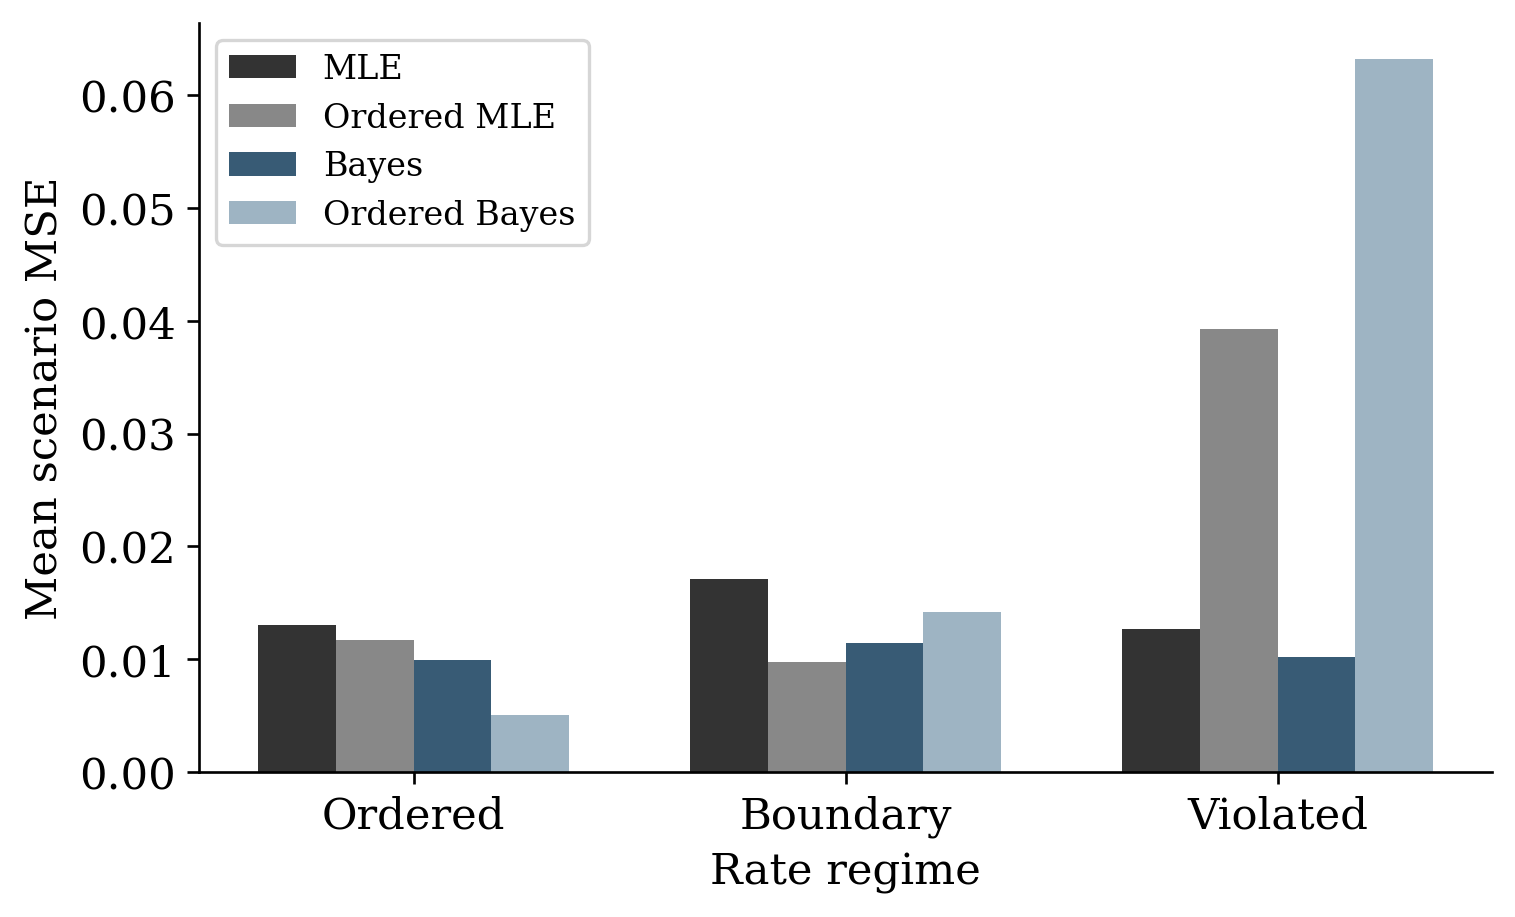
\includegraphics[width=.82\linewidth]{simulation_mse.png}
\caption{Mean scenario-specific MSE for reliability. Each bar averages 16 scenarios in one rate regime.}\label{fig:mse}
\end{figure}
At the equality boundary, ordered equal-tail intervals have coverage 0.000, whereas ordered numerical HPD intervals have coverage 0.914. Their mean widths are 0.253 and 0.233, respectively. The HPD calculation allows the lower endpoint to equal one half. This explains why its boundary coverage differs from the equal-tail result; it does not establish nominal coverage in every scenario.


Ordered MLE bootstrap coverage is assessed separately in six selected scenarios, with 100 outer datasets and 199 bootstrap resamples each. This smaller comparison has larger Monte Carlo uncertainty. It does not assign a regular normal interval to a boundary estimate.
\begin{table}[htbp]
\centering
\caption{Ordered MLE bootstrap intervals in six selected scenarios: 100 outer datasets and 199 resamples per dataset. MCSE refers to coverage.}\label{tab:bootstrap}
\small
\begin{tabular}{llrrr}
\toprule
Rate regime & Protocol & CP & MCSE & AW \\
\midrule
Ordered & Type I & 0.910 & 0.029 & 0.371 \\
Ordered & Adaptive II & 0.860 & 0.035 & 0.364 \\
Boundary & Type I & 0.940 & 0.024 & 0.340 \\
Boundary & Adaptive II & 0.910 & 0.029 & 0.343 \\
Violated & Type I & 0.000 & 0.000 & 0.321 \\
Violated & Adaptive II & 0.000 & 0.000 & 0.306 \\
\bottomrule
\end{tabular}
\end{table}


\subsection{Real data analysis}\label{sec:data}
The examples use published breaking-strength measurements. Both strength and comparison stress are measured in the same units within an example. The comparison group is a laboratory reference population, not a set of measured operating loads. The calculated reliability should therefore not be described as a certified in-service probability.

\subsubsection{Jute-fibre measurements}
The 15 mm and 20 mm jute-fibre groups have 30 observations each. They are transcribed, in printed order, from Table 10 of Sultana et al.\ \cite{Sultana2026}, where they are attributed to Xia et al.\ \cite{Xia2009}. The reproduced measurements have already been divided by 1000. We use 15 mm as strength and 20 mm as comparison stress. The 10 mm group is excluded because the reproduced table contains the unverified value 70.32383. We do not guess a replacement for it. The original Xia experimental file was not available; the supplied secondary table is the transcription source.

We first fit the complete groups and assess Weibull fit using bootstrap-calibrated Kolmogorov-Smirnov tests with refitting in each of 1000 resamples. We also test the common-shape assumption by a bootstrap likelihood-ratio test. Fitted-parameter K-S tests need this calibration; ordinary distribution-free K-S p-values would not apply.
\begin{table}[htbp]
\centering
\caption{Complete-data Weibull fits and bootstrap-calibrated K-S tests. Carbon rates use the fixed 3 GPa measurement unit.}\label{tab:gof}
\small
\begin{tabular}{lrrrrr}
\toprule
Sample & $n$ & $\widehat\alpha$ & Rate & K-S & $p$-value \\
\midrule
Jute strength & 30 & 1.499 & 3.908 & 0.169 & 0.026 \\
Jute comparison & 30 & 1.361 & 3.839 & 0.149 & 0.078 \\
Carbon strength & 50 & 2.719 & 1.180 & 0.078 & 0.585 \\
Carbon comparison & 50 & 2.897 & 0.942 & 0.113 & 0.101 \\
\bottomrule
\end{tabular}
\end{table}

For the jute groups, the common-shape bootstrap p-value is 0.620. The calibrated K-S p-values are 0.026 and 0.078. Thus the first group rejects Weibull adequacy at 5 percent, even though the common-shape test does not reject. The jute estimates must be read with this fit limitation. The carbon common-shape bootstrap p-value is 0.678. Table~\ref{tab:gof} reports its separate fit checks.

\begin{figure}[htbp]
\centering
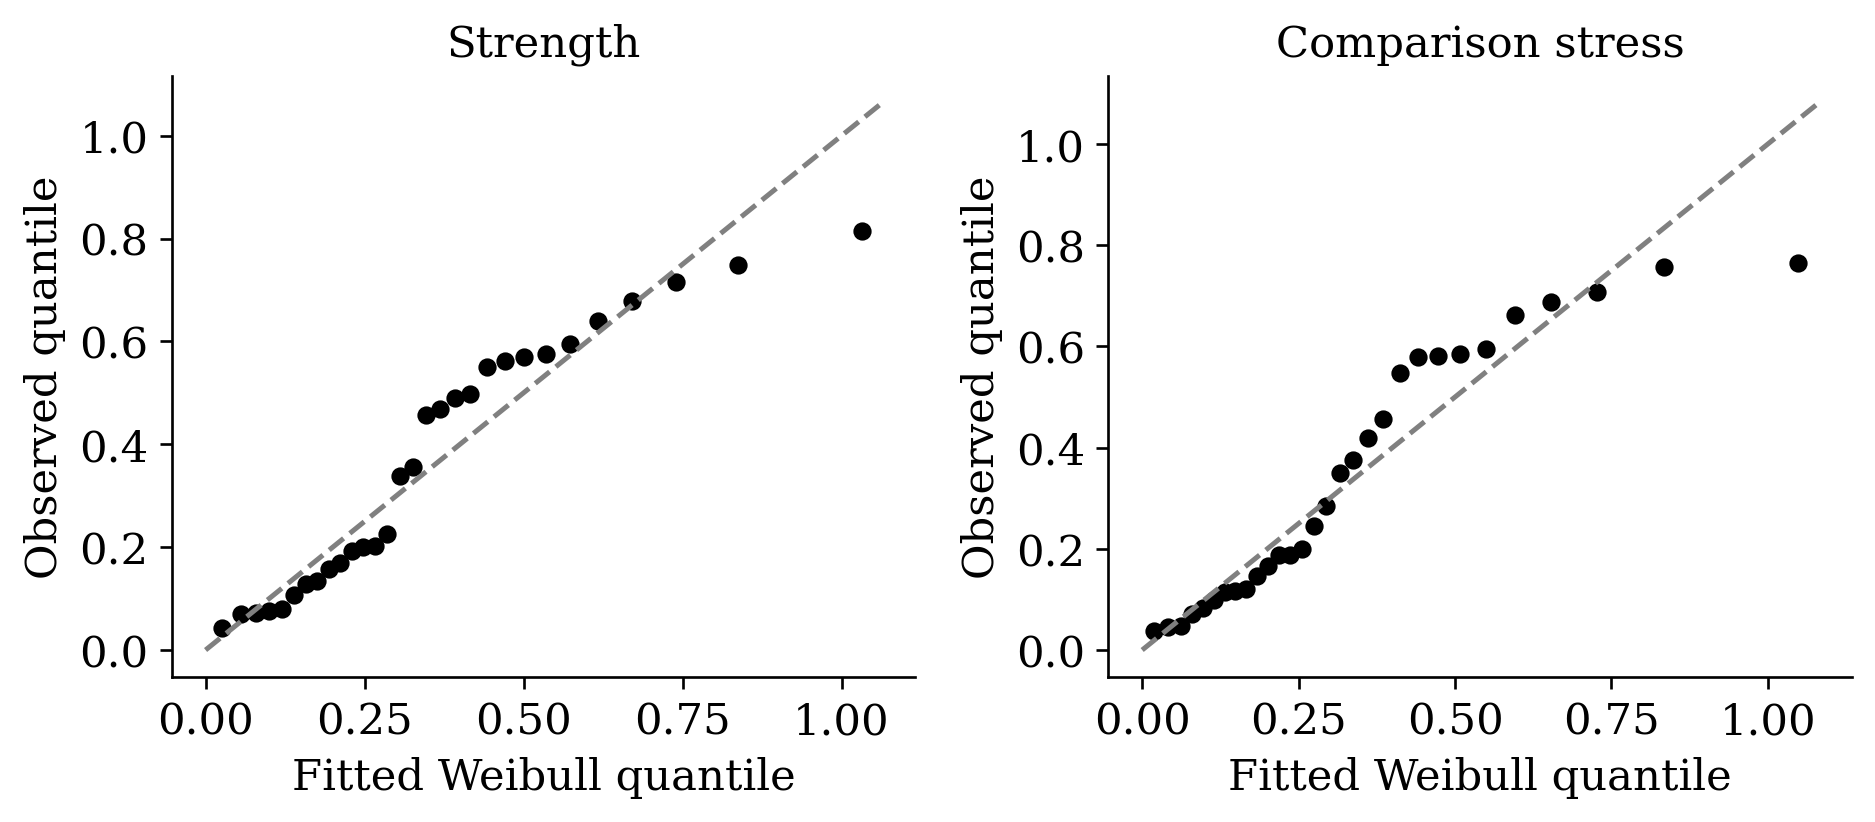
\includegraphics[width=.96\linewidth]{jute_qq.png}
\caption{Weibull Q-Q plots for the complete jute groups. A fitted model would place observations approximately along the diagonal.}\label{fig:jute-qq}
\end{figure}

Next, a seeded allocation divides the strength group into three blocks of ten. Each block has target seven failures, balanced withdrawals and $T=0.5$. Type-I progressive hybrid censoring leaves 13 observed failures altogether. From the comparison group we retain the first six upper 2-records, stopping at position nine. The printed order is an imposed acquisition order; it is not known to be the historical order of the measurements. The notebook examines alternative random orders as a sensitivity check. Allocation, withdrawals, terminal survivors and record positions are saved in the data folder.

\subsubsection{Additional carbon-fibre measurements}
Because of the jute fit limitation, we also use the 100 carbon-fibre measurements reproduced by Newer and Alanazi \cite{NewerAlanazi2026}, Section 5.1.1, attributed there to Nichols and Padgett \cite{Nichols2006}. They are in GPa. A seeded random permutation splits them into disjoint groups of fifty. We divide both groups by a fixed 3 GPa unit before inference, and keep the same prior hyperparameters on these scaled rates. The original Nichols and Padgett experimental file was not supplied; the reproduced article is the source for our transcription.

Strength block sizes are 17, 17 and 16, with target $\lfloor0.7n\rfloor$, $T=1$ in scaled units and balanced withdrawals. We use the first five upper 4-records from the comparison half. The retained records are distinct, so no jitter is added to rounded source values. Both complete groups are compatible with the fitted Weibull distributions at the 5 percent level, and the common-shape test does not reject. This supports using the carbon example as an additional illustration, without proving the assumptions true.
\begin{figure}[htbp]
\centering
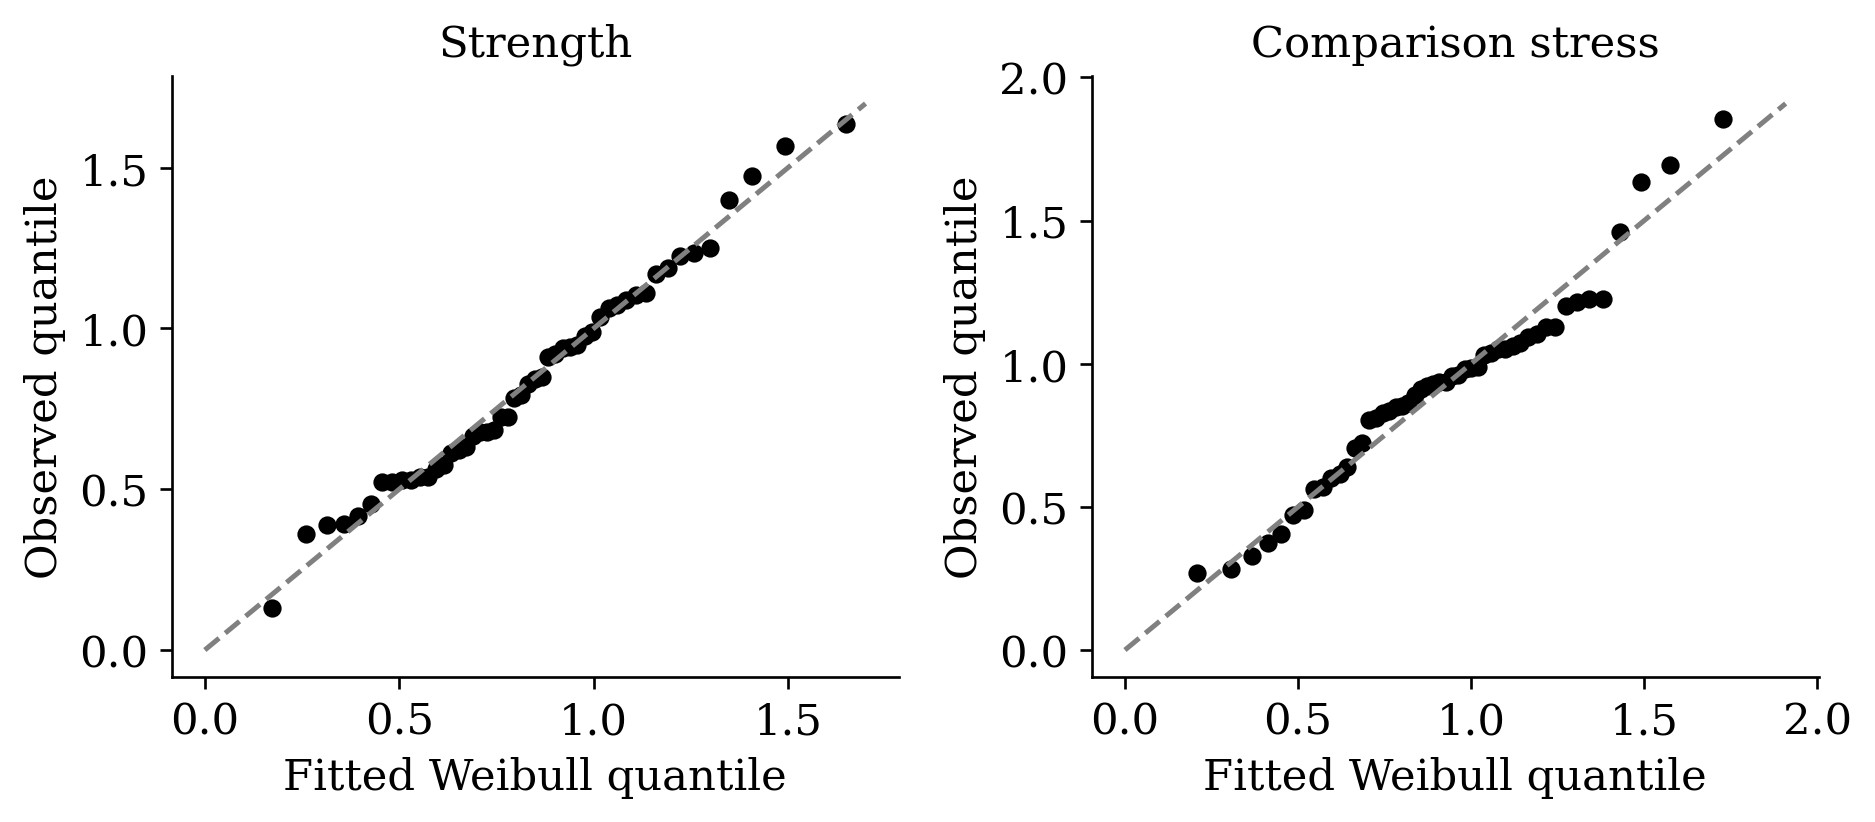
\includegraphics[width=.96\linewidth]{carbon_qq.png}
\caption{Weibull Q-Q plots for the two randomly allocated carbon-fibre groups. Measurements are expressed in units of 3 GPa.}\label{fig:carbon-qq}
\end{figure}

\begin{table}[htbp]
\centering
\caption{Parameter and reliability estimates with 95 percent reliability intervals. Interval types are explained in the text.}\label{tab:real-estimates}
\small
\begin{tabular}{llrrrrl}
\toprule
Data & Estimator & $\alpha$ & $a$ & $b$ & $R$ & 95 percent interval \\
\midrule
Jute & MLE & 1.166 & 2.117 & 4.846 & 0.753 & [0.444, 0.945] \\
Jute & Ordered MLE & 1.166 & 2.117 & 4.846 & 0.753 & [0.500, 0.947] \\
Jute & Bayes & 1.179 & 2.201 & 3.901 & 0.666 & [0.380, 0.895] \\
Jute & Ordered Bayes & 1.165 & 2.104 & 4.127 & 0.699 & [0.516, 0.899] \\
Carbon & MLE & 2.874 & 1.341 & 0.695 & 0.316 & [0.133, 0.615] \\
Carbon & Ordered MLE & 2.660 & 1.135 & 1.135 & 0.500 & [0.500, 0.862] \\
Carbon & Bayes & 2.784 & 1.317 & 0.827 & 0.362 & [0.159, 0.608] \\
Carbon & Ordered Bayes & 2.552 & 1.080 & 1.338 & 0.565 & [0.502, 0.704] \\
\bottomrule
\end{tabular}
\end{table}

\begin{table}[htbp]
\centering
\caption{Numerical 95 percent HPD intervals for reliability in the data examples. The probability column checks mass under the interpolated posterior density.}\label{tab:real-hpd}
\small
\begin{tabular}{lllrr}
\toprule
Data & Posterior & HPD interval & Width & Probability \\
\midrule
Jute & Unrestricted & [0.4040, 0.9115] & 0.5075 & 0.950 \\
Jute & Ordered & [0.5000, 0.8744] & 0.3744 & 0.950 \\
Carbon & Unrestricted & [0.1462, 0.5915] & 0.4454 & 0.950 \\
Carbon & Ordered & [0.5000, 0.6752] & 0.1752 & 0.950 \\
\bottomrule
\end{tabular}
\end{table}

Table~\ref{tab:real-estimates} uses a log-ratio asymptotic interval for the unrestricted MLE, a 500-resample percentile bootstrap interval for the ordered MLE, and equal-tail intervals for the Bayesian rows. Table~\ref{tab:real-hpd} gives the numerical HPD alternatives for the same posterior distributions. Confidence intervals and posterior credible intervals have different interpretations.

\begin{figure}[htbp]
\centering
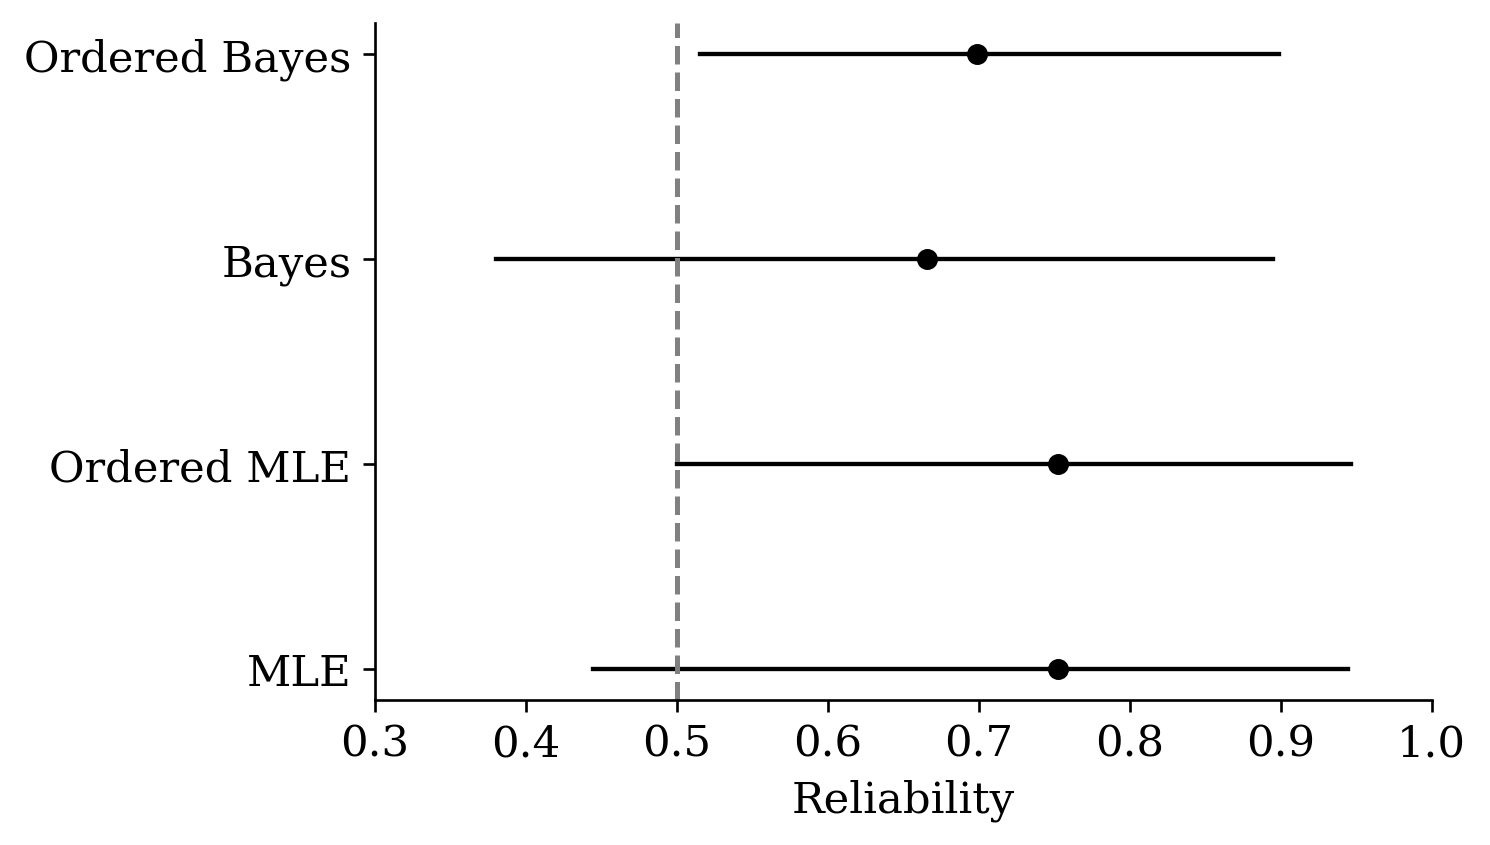
\includegraphics[width=.82\linewidth]{jute_intervals.png}
\caption{Jute reliability estimates and their 95 percent intervals from Table~\ref{tab:real-estimates}. The dashed line is the ordered model's lower bound.}\label{fig:real-intervals}
\end{figure}
The jute estimates illustrate the calculation, but the rejected fit in one group must remain part of their interpretation. The carbon results are also sensitive to imposing an order: the ordered model excludes every reliability below one half. A narrower interval in that model is partly a consequence of the assumption, rather than evidence that the assumption is correct.

\section{Conclusion}\label{sec:conclusion}
We derived the shared-stress reliability of a Weibull $s$-out-of-$K$ system and used the appropriate likelihood for block progressive hybrid strengths and upper k-record stresses. Both unrestricted and ordered MLEs were obtained by profiling over the common shape. A dependent gamma-Dirichlet prior gave Bayesian estimates in both cases, with numerical integration reducing the posterior calculation to two dimensions.

The simulation compares point-estimation errors and the coverage and width of asymptotic, equal-tail and numerical HPD intervals. The ordered Bayesian estimates perform well in the correctly ordered cases studied here. A false restriction produces substantial bias, and intervals constrained above one half cannot cover a reliability below one half. At the equality boundary, HPD and equal-tail intervals behave differently because an HPD interval may include the boundary itself.

Published measurements provide reproducible illustrations, rather than proof of engineering performance. The jute example has a documented fit problem; the carbon example gives a compatible additional validation. The common-shape assumption, noninformative withdrawals and the imposed record acquisition order are limitations. The notebook includes prior and acquisition-order sensitivity checks and posterior diagnostics. Future work could study unequal shapes or other withdrawal plans, but those extensions are outside the present project.

\begingroup
\small
\bibliographystyle{IEEEtran}
\bibliography{reference}
\endgroup
\end{document}
